\documentclass[10 pt]{article}
\usepackage{graphicx}
\pagestyle{plain}
\usepackage[OT4]{polski}
\usepackage[utf8]{inputenc}
\title{Sprawozdzanie 10 \\ \emph{\textbf{A star }}}
\author{Paweł Żurek 200404}
\date{29.05.2014}
\begin{document}
\tableofcontents
\maketitle
\section{Wstęp}
Prosty program, w którym można przetestować działanie algorytmu \textbf{A star}.
\section{Krótki opis programu}
\textbf{Program po uruchomieniu pyta się z ilu wierzchołków ma stworzyć graf a następnie : }
\begin{itemize}
\item Pyta się w jakim miejscu postawić przeszkodę
\item Pyta się o współrzędne punktu początkowego
\item Pyta się o współrzędne punktu końcowego
\item Wyświetlenie graficzne działania algorytmu
\end{itemize}
Graf jest przedtawiony jako układ współrzędnych, gdzie punkty to wierzchołki. Układ ten zawsze jest kwadratowy, tzn szerokość i długość takie same.

\section{\textbf{DFS} vs \textbf{BFS} vs \textbf{A star}}
Działanie algorytmów BFS i DFS opisałem dokładniej w sprawozdaniu numer 8.
\\
Algorytm \textbf{A*} wywolywany jest bezparametrycznie, jednak przy konstrukcji grafu ustalamy pozycje wierzchołka początkowego jak i szukanego.
\subsection{Wyniki : }
\begin{center}
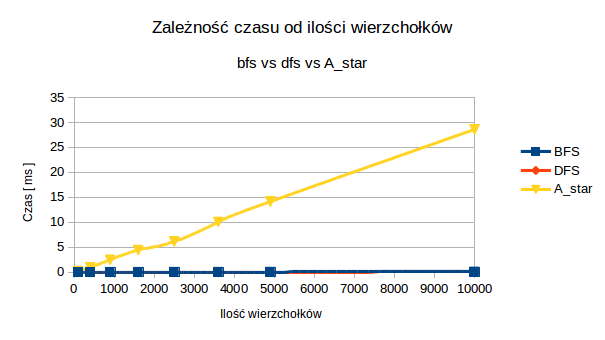
\includegraphics[scale=0.7]{wykres.png}
\end{center}
\begin{center}
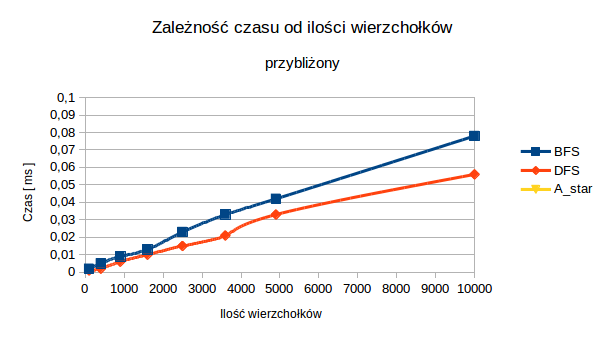
\includegraphics[scale=0.7]{wykres_przyblirzony.png}
\end{center}
\subsection{Uwagi :}
\begin{itemize}
\item Zarówno algorytm \textbf{bfs} jak i algorytm \textbf{dfs} uruchamiałem z tym samym argumentem : wierzchołkiem o numerze 1.
\item Algorytm \textbf{A star} uruchamiałem zawsze dla wierzchołka początkowego odpowiadającemu punktowi (\textbf{0},\textbf{0}) oraz dla wierzchołka końcowego odpowiadającemu punktowi (\textbf{rozmiar-1}, \textbf{rozmiar-1} )
\end{itemize}
\section{Algorytm \textbf{A*}}
Algorytm jest zupełny i optymalny, w tym sensie, że znajduje ścieżkę, jeśli tylko taka istnieje, i przy tym jest to ścieżka najkrótsza. Stosowany głównie w dziedzinie sztucznej inteligencji do rozwiązywania problemów i w grach komputerowych do imitowania inteligentnego zachowania.
\section{Wnioski:}
\begin{itemize}
\item Pomimo faktu, iż algorytm \textbf{A star} jest jednym z bardziej rozbudowanych algorytmów wyszukiwania, daje całkiem niezłe wyniki czasowe. Oprócz czasu, nie można zapominać, iż algorytm ten znajduje najlepszą scieżkę ! W przeciwieśwtie do innych algorytmów tego typu ( np. \textbf{Dijkstry}),
\item W porównaniu do algorytmów \textbf{DFS} i \textbf{BFS} okazał się znacznie wolniejszy. Powodem tego, może być : 
\begin{itemize}
\item Złożoność algorytmu \textbf{A star}. Głownie zwiększa ją heurystyka,
\item Błąd w liczeniu czasów \textbf{DFS} i \textbf{BFS}. Liczę te czasy tymi samymi metodami. Wyniki może nie są nie logiczne, lecz jak na mój gust zbyt optymistyczne.
\end{itemize}
\item Algorytm \textbf{A*} jest prawdopodobnie najefektywniejszym algorytmem tego typu. Dzieje się tak głównie poprzez fakt, iż algorytm na bieżąco ''przewiduje'', która ścieżka jest optymalna.  
\end{itemize}

Dokładne wyniki programu są zamieszczone w pliku ( obecny folder ) \textit{dane.xls}. Podobnie wszystkie wykresy są dostępne w osobnych plikach ( format png ). Dodatkowo w aktualnym folderze dostępna jest dokumentacja wygenerowana w \LaTeX u oraz w DoxyGen 'ie.

\end{document}